\section{Model}
In this section, each part of the model is discussed. On figure \ref{fig:GA_MODEL} a general overview of the model is illustrated. Before we go into detail, we briefly discuss the different components of our model.
\begin{figure}
    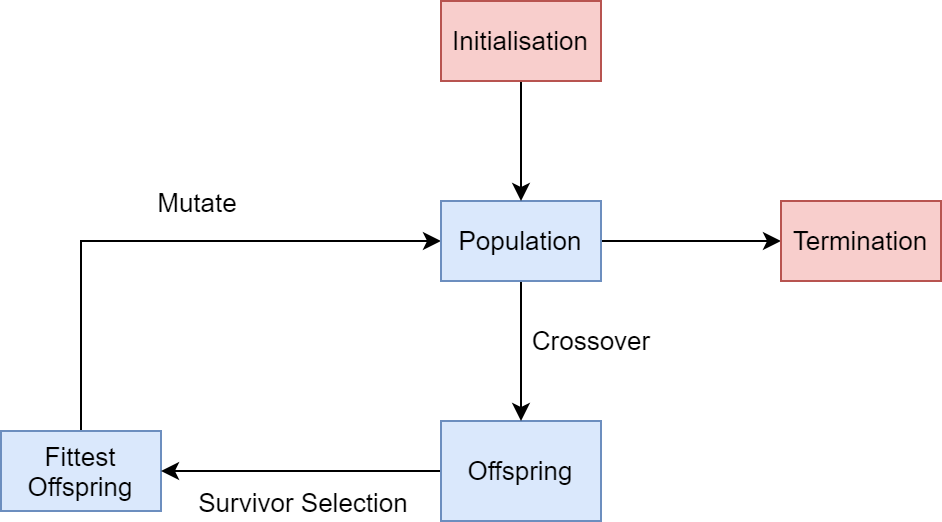
\includegraphics[width=\linewidth]{figures/GA_structure.png}
    \caption{The genetic model, an overview of the important components.}
    \label{fig:GA_MODEL}
\end{figure}

The initial population can consist of both random songs or non-random songs, these are called $GEN0$. The next generation is calculated by applying a crossover function on $GEN0$ to obtain $GEN1$ which is the offspring. Each individual song in the offspring will be rated by the fitness function and obtains a score. Now we can select the best rated songs in $GEN1$ and mutate them. This process is repeated until a certain condition is met or until user is satisfied with the results and manually terminates the loop.
\section{Initialization}
First, the initial population needs to be determined, we call it $GEN0$ throughout this paper. $GEN0$ usually consist of a mix of different songs from different genres making the initial population diverse. The size of the population, which is static during the execution, is decided here and is related to the number of parents. %TODO reference to next section or not?
\section{Recombination}
In the recombination step, a crossover function is used to pair parents in order to produce a child. This child will belong to the next generation. The model performs a uniform crossover, meaning each gene will be considered separately when pairing the parents \cite{BOOK:GA}. For each song, the notes, chords and rests are considered as the genes of a song. Two parents produce only one child by uniformly selecting genes from one of the two parents. 
On figure \ref{fig:cross_init}, an example of two songs, that are considered as parents, are graphically displayed. During the crossover process, the model iterates over all the genes in both parents and selects only one or the other to pass to the resulting child. Both genes have an equal chance of being selected. On figure \ref{fig:cross_7} a sample child of the corresponding parents is illustrated.
\begin{figure}[H]
    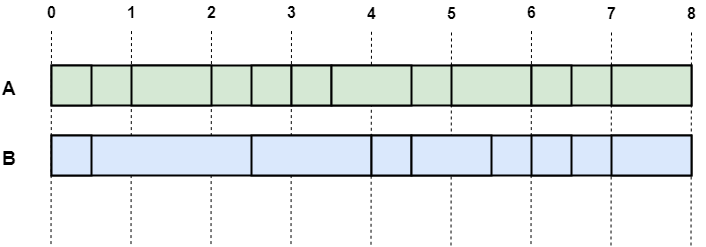
\includegraphics[width=\linewidth]{Fotos/crossover/init.png}
	\caption{Graphical display of two parents A and B. Each rectangle represents a note, chord or rest with their corresponding length. The horizontal axis represents time.}
	\label{fig:cross_init}
\end{figure}
\begin{figure}[H]
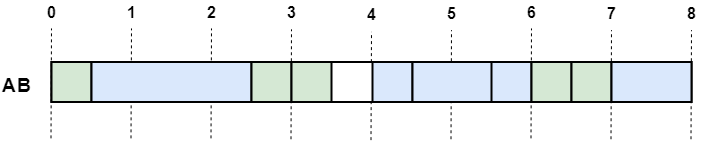
\includegraphics[width=\linewidth]{Fotos/crossover/last.png}
\caption{The child generated from the parents A and B.}
\label{fig:cross_7}
\end{figure}
Notice that there is a gap in the child song at time offset $3.5$. This is the result of selecting parent B's gene at time offset $4$ instead of the corresponding gene of parent A's at time offset $3.5$. 

At each recombination step, all the parents are paired with each other. If there are \(N\) parents, the number of children will be equal to \( \frac{N * (N-1)}{2} \). After the recombination, the fitness of each child will be calculated.

\subsection{The fitness function}
A composition has multiple aspects that can be rated at each individual level, therefore, the fitness of an individual is determined by different \textbf{rating functions}. Each of these rating functions gives a certain \textbf{score} for a particular \textbf{concept} of the song. We clarify with an example: the tendency to follow a musical scale within the composition can be such a concept. Every rating function calculates a score and to this score there is a predetermined weight attached that implies the importance of the rated concept. The total fitness of a song $x$ is equal to the sum of the products of all rating functions S for each concept and their corresponding weights W.
\[ TotalFitness(x) = \sum_{i=1}^{C} S_{i} * W_{i}\] 
where C is the number of concepts.


\[ S(x) =  difference( f(x) ,optimalscore) * S_{weight} \]

\subsubsection{The master song}
The fitness function calculates a score song based on the master. The master song is set during the initialisation process and it controls the population by defining the rules. We can rate candidate songs based on the master song in two ways:
\begin{itemize}
    \item absolute comparison: this is where we compare the elements of the master song directly with the candidate song.
    \item relative comparison: this is where we compare the relative structure of the master song directly with the candidate song.
\end{itemize}


\section{Survivor selection}
% TODO explain survivor selection
After 
\\
